\chapter{Literature Review}\label{c:literature}

\section{Optrode system}

In recent years, optrode technology has been invented and used to interface with brains.  Compared to traditional electrodes, optrode can be more precise, take less tissue damage \cite{MoreOptrode_5}, and be able to simultaneously stimulate and record.  The light source of the optrode can be external \cite{MoreOptrode_6}\cite{MoreOptrode_7}, or integrated on the optrode \cite{MoreOptrode_8}\cite{MoreOptrode_2}.  As the optrodes are getting smaller, they can be manufactured into arrays \cite{MoreOptrode_1}\cite{MoreOptrode_3}, or even 3-dimensional arrays \cite{MoreOptrode_4}, which can cover a larger area or volume of tissue, enabling the study of network dynamics \cite{MoreOptrode_9} or interactions between different brain regions \cite{MoreOptrode_10}.  The size and power consumption of optrode systems can be small enough to fit in a portable device \cite{MoreOptrode_11}, which would be beneficial for brain-machine interfaces.

\subsection{Existing optrode system}
In this project, we are working on improving the noise performance of an existing optrode system \cite{OptrodeProceesings} (shown in fig.~\ref{fig_OptrodeFigure}).  A superluminescent diode emits light to a circulator, which directs the light to a liquid crystal transducer.  The transducer receives nerve activity signal from the two electrodes.  This causes the change of liquid crystal angle, which then changes the reflection rate of the light.  Therefore, the nerve activity message is modulated to the light and the light is reflected to the circulator, which then directs the light to a photodiode light detector.  This detector converts the light signal to a current signal, and eventually the current signal is converted to digital data via an amplifier circuit and data acquisition equipment. 

\section{Active noise cancelling}

\subsection{Wiener filter}

\begin{figure}[H]
\centerline{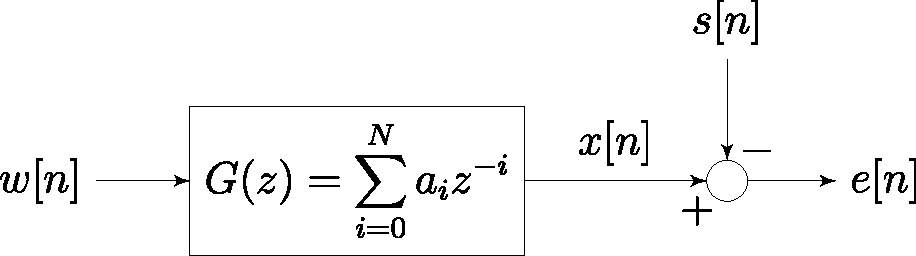
\includegraphics[scale=0.5]{3-literature/Wiener_block.pdf}}
\caption{Wiener filter block diagram, $s[n]$ is a noise free signal, and $w[n]$ is $s[n]$ plus some noise.  $w[n]$ is inputted to the filter, $G(z)$ is the Wiener filter, and $x[n]$ is the filter output.  $e[n]$ is the error between $x[n]$ and $s[n]$, the Wiener filter should try to minimize $e[n]$}
\label{fig_Wiener_block}
\end{figure}

To reduce the noise in the system, an active noise reduction algorithm is needed.  The Wiener filter is one of the choices when dealing with two channel noise reduction.  A FIR Wiener filter for discrete signals \cite{WienerPaper} is shown in fig.~\ref{fig_Wiener_block}, $s[n]$ is a noise free signal, and $w[n]$ is $s[n]$ plus some noise.  $G(z)$ is the Wiener filter with $a_i$ being the filter coefficients.   $w[n]$ is inputted to the filter, and $x[n]$ is the filter output.  $e[n]$ is the error between $x[n]$ and $s[n]$.  From this diagram, the mean square error is:
$E[e^2 [n]]=E[(x[n]-s[n])^2]$

After expanding the equation above, a matrix equation came out with $a$ to be the coefficients that minimise the mean square error:


\begin{gather} \label{eqn_WienerMatrix}
\underbrace{
    \begin{bmatrix}
    R_w[0] & R_w[1] & \dots & R_w[N] \\
    R_w[1] & R_w[0] & \dots & R_w[N-1] \\
    \vdots & \vdots & \ddots & \vdots \\
    R_w[N] & R_w[N-1] & \dots & R_w[0]
    \end{bmatrix}
}_{T}
\underbrace{
    \begin{bmatrix}
    a_0 \\
    a_1 \\
    \dots \\
    a_N
    \end{bmatrix}
}_{a}
=
\underbrace{
    \begin{bmatrix}
    R_{ws}[0] \\
    R_{ws}[1] \\
    \dots \\
    R_{ws}[N]
    \end{bmatrix}
}_{v}
\end{gather}

In eqn~\ref{eqn_WienerMatrix} the matrix $T$ is the autocorrelation of $w[n]$, and inside the matrix $v$ is the cross correlation of $w[n]$ and $s[n]$, where both $w[n]$ and $s[n]$ is known.  Therefore, both matrix $T$ and $v$ are known, so matrix $a$ can be calculated, which is the filter coefficients.
This method uses a noise free message signal $s[n]$ and a noisy message signal $w[n]$ as input, and the filter reduces the noise inside $w[n]$.  This is different to how the noise reduction algorithm would work in this project.  From the optrode system, a noisy message signal and a pure noise signal can be extracted, while the pure noise signal is highly correlated to the noise inside the noise message signal.  To use the Wiener filter, the pure noise signal can be the input $w[n]$ and the noisy message signal can be the input $s[n]$.  The output $x[n]$ would be the correlated noise between the pure noise signal and the noisy message signal.  Then, subtract $x[n]$ from $s[n]$ to give the signal after noise reduction.
For two long discrete signals, say a \qty{10}{s} signal with a sampling rate of \qty{100}{kHz}, each signal has one million samples.  For matrix $T$, that means a one million times one million size, which takes a huge amount of computational power.  The plan is to run this algorithm on an FPGA, which cannot handle this task.  Also, it is desired to have real-time output with low latency.  The Wiener filter is very hard to achieve both high noise reduction rate and low latency since the filter needs a fair number of samples to work.
In conclusion, the Wiener filter is a good algorithm to start with.  however, it cannot suit all the requirements for this project, so modifications and other methods must be considered.



\subsection{ANC on audio systems}

Active noise cancelling technique is widely used in audio systems.  It can help remove noise from human ears either using a headset \cite{ANC_Headphone_10} or a larger speaker \cite{ANC_Car}.  There are a few ways to achieve noise cancelling with a headset, such as using a microphone at the outside of the headset to capture noise and feedforward \cite{ANC_Headphone_8} to algorithms to process, and output the anti-sound using the headset speaker.  Alternatively, the microphone can be placed inside the headset to feedback \cite{ANC_Headphone_5} noise sound and then cancel it with the speaker sound.  It is also very common to use both feedforward and feedback at the same time \cite{ANC_Headphone_4}.  
A lot of headset active noise cancelling processes \cite{ANC_Headphone_1}\cite{ANC_Headphone_2} are using Filtered-X Least Mean Squares (FxLMS) algorithm \cite{ANC_Headphone_7}, or the modified version of it \cite{ANC_Headphone_9}\cite{ANC_Headphone_6}.

The FxLMS algorithm is an advanced version of the standard Least Mean Squares (LMS) algorithm tailored for active noise cancelling. ANC aims to diminish unwanted noise by producing an ``anti-noise'' sound wave that counteracts the undesired noise. A challenge in ANC is the secondary path between the speaker, which emits the anti-noise, and the error microphone, which gauges noise cancellation effectiveness; this path can introduce delays and distortions. The FxLMS algorithm addresses this \cite{ANC_Headphone_11} by first filtering the reference noise signal through a model of the secondary path, creating the ``Filtered-X''. Then, using this filtered-X signal and the error signal from the microphone, the LMS algorithm adaptively updates the filter weights to minimize the difference between the desired signal (typically silence) and the adaptive filter's output. This continuous adaptation allows the FxLMS algorithm to control noise in dynamic environments.

\section{Digital signal processing on FPGA}

\begin{figure}[h]
\centerline{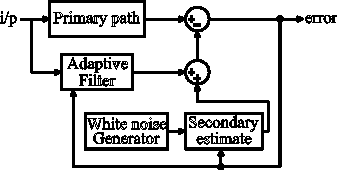
\includegraphics[width=0.6\linewidth]{3-literature/ANCHeadphoneFPGA.pdf}}
\caption{Block Diagram for an active noise cancelling system.}
\label{fig_ANCHeadphoneFPGA}
\end{figure}

A block diagram for active noise cancellation algorithm on FPGA \cite{ANC_Headphone_3} is shown in fig.~\ref{fig_ANCHeadphoneFPGA}.  The high-level design is basically a negative feedback control loop with inputs being reference microphone and error microphone, and output being sound data after noise reduction.  The feedback is connected to an adaptive filter that uses the filtered-x least mean square (FxLMS) algorithm.  The coefficients are calculated by the previous coefficients, input data, and feedback error signal inside a weight update controller.  It keeps updating the coefficient until the error signal goes to zero.  Inside the adaptive filter, there are 24 filter taps.  There are results showing that after the 17h filter tap, the coefficients are very close to zero.  Also, a comparison was made showing that 24 filter taps and 60 filter taps achieve the exact same noise reduction ability, while 60 filter taps have 200\% more computational complexity.  Therefore, 24 is an appropriate number of filter taps that does not use too many resources but still maintains decent noise reduce ability.  A pipeline structure is also designed to reduce the hardware resources used.  As high frequency noise can be largely reduced by passive noise control, active noise cancellation only needs to work at lower frequencies, for instance, lower than 1kHz.  Modern FPGAs can run at around \qty{100}{MHz} frequency, which is a lot faster than the required sound frequency.  In this case, 24 filter taps are being pipelined, which means for each sample period the filter is running 24 times to get 24 filter taps.  A single 24-Filter unit structure as well as the pipelined single-multiplier filter have been implemented to compare the resource utilization rate.  The result shows that the non-pipelined filter cost 77\% of slice look up tables (LUTs) and 425\% of bonded input output blocks (IOBs) on the FPGA, and the pipelined filter cost 13\% of slice LUTs and 34\% of bonded IOBs.  It is not a 24 times difference since the pipelined filter is only part of the whole design.  However, it is still very significant as the non-pipelined design uses almost all the slice LUTs and 4 times the IO pins onboard, which means it is impossible to implement on the actual FPGA.

It is mentioned in this paper that the algorithm focuses on frequencies under \qty{1}{kHz}.  This is not only because passive noise control can handle the high frequency noise, but also active noise cancellation hardware now cannot deal with high frequency very well.  The algorithm and hardware need time to capture, process, and output.  Which means there must be a time delay between the input noise and the output cancelling noise.  This time delay may cause only a small phase shift at lower frequencies, but it would be very serious at higher frequencies, which leads to a failure to cancel or even add more noise.  For our project, the required working frequency range is about the same as audible sound, but does not have a strict time delay requirement, because we do not need to race with the speed of sound, which means similar hardware and algorithm should satisfy the requirements of our project (or even higher than requirements of our project).  The filter length result suggests that there is a filter tap number after which the noise reduction ability will not change.  The optrode system data shows that the noisy signal and noise signal are only correlated for about 7 samples, so it is safe to assume that the noise reduction ability would reach its maximum at 7 filter taps.  This paper also discussed pipeline techniques, which could be very useful in this project.  In this project, more data bits may be used for higher accuracy, which means a lot more resources will be taken.  By using a pipeline structure, hardware cost is converted to time cost.  Since the FPGA runs at a much higher frequency than the signal of interest, it is safe to run multiple times within a sample period.

\section{Photodiode}

In this project, we need to build a new PCB (a light receiver board) that converts analogue light signal into digital signal for the FPGA to process.  The input power to the light source in the existing optrode system just exceeds \qty{22.5}{mW} \cite{OptrodePower}.  We will be using the same photodiode from the existing optrode system from Flyin \cite{Flyin}, which has a responsivity of \qty{0.9}{A/W}.  We can then calculate the current output from the photodiode will be around $\qty{22.5}{mW}/(\qty{0.9}{A/W})=\qty{25}{mA}$.  However, in the actual system, due to the light circuit configuration, the light loss in the light circuit, and the amount of light being modulated in the optrode, experiment shows only a few microamps current coming out of the photodiode.  At this current level, we need to be very careful of the noise generated by the components around the photodiode, as they can easily making the signal to noise ratio bad.

With the optrode system, the liquid crystal transducer modulates the nerve signal into the lights by changing the amount of light being reflected.  However, it only modulates less than 10\% of the light, which means the AC part of the light is far less than the DC part.  This may cause problems with the light receiver part of the system.

\begin{figure}[h]
\centerline{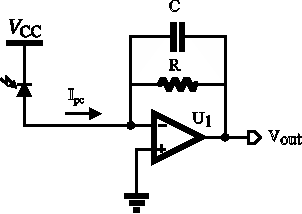
\includegraphics[width=0.6\linewidth]{3-literature/ReverseBiasSch.pdf}}
\caption{A reverse-biased photodiode circuit schematic.  The photodiode current $I_{pc}$ is amplified by a transimpedance amplifier.}
\label{fig_ReverseBiasSch}
\end{figure}

A common way to use a photodiode as light detector is to use it in photoconductive mode.  In photoconductive mode, the photodiode is reverse biased \cite{PDbook}, which means the anode has been given a voltage lower than the cathode.  Fig.~\ref{fig_ReverseBiasSch} shows a reverse-biased photodiode circuit schematic.  A transimpedance amplifier is connected to the cathode of a photodiode to convert and amplify the output current to a voltage signal.  This is a good choice when it is needed for the output signal relevant to illuminance.  However, when only the AC part is needed, and the AC part is very small compared to the DC part, this DC-coupled detect-amplify circuit must lower the gain to avoid saturation.  This means the gain in the subsequent AC coupled amplifier has to rise, and therefore the noise for this stage is no longer negligible, which means an increased input-referred noise.

One way to remove the DC part in the signal is to use a DC feedback loop \cite{IOffsetTIA}.  Fig.~\ref{fig_IFeedbackSch} shows an active DC photocurrent cancellation circuit, it uses a differential transimpedance amplifier to amplify the photocurrent received by the photodiode, then uses an error amplifier along with a MOSFET to feedback the DC current into the negative input of the differential amplifier to actively remove the DC current part of the photocurrent.

\begin{figure}[h]
\centerline{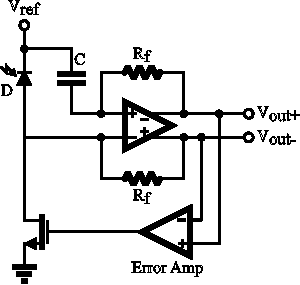
\includegraphics[width=0.6\linewidth]{3-literature/IFeedbackSch.pdf}}
\caption{Active DC photocurrent cancellation circuit. The error amplifier controls the MOSFET to drain the same amount of current as the DC current of the diode.}
\label{fig_IFeedbackSch}
\end{figure}

Another way to remove the DC signal is to use another configuration to operate photodiodes \cite{zero-mode_detection}, which results in higher AC gain in the transimpedance amplifier and lower noise.  This mode is called “zero mode”, and it forces the photodiode to operate at either zero voltage or zero current.  

\begin{figure}[h]
\centerline{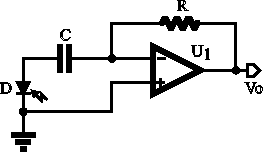
\includegraphics[width=0.6\linewidth]{zero_mode_sch.pdf}}
\caption{Zero-mode configuration with capacitor AC coupling the input.}
\label{fig_zero_mode_sch}
\end{figure}

\begin{figure}[h]
\centerline{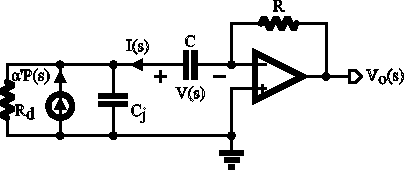
\includegraphics[width=0.8\linewidth]{3-literature/ZeroModeSS.pdf}}
\caption{zero-mode Small AC signal equivalent circuit}
\label{fig_ZeroModeSS}
\end{figure}

Fig.~\ref{fig_zero_mode_sch} shows a proposed circuit design that the photodiode is working in zero-mode.  Experiments are done to measure the parameters of the photodiode in zero-mode, such as the saturation current, the ideality factor, the slope indicator, and the power to current conversion efficiency.  With these parameters, a small AC signal equivalent circuit (shown in fig.~\ref{fig_ZeroModeSS}) can be derived.  

The transfer function can be derived:

$$H(s) = \frac{V_0}{P} = - \frac{\alpha'RsCR_d}{1+s(C+C_j)R_d}\frac{1}{1+s/\omega_0} = - \frac{\alpha'RC}{C+C_j} \frac{s}{s+\omega_c} \frac{\omega_0}{s+\omega_0}$$

$$\omega_c = \frac{1}{(C+C_j)R_d}$$


The transfer function of this circuit indicates that it works as a bandpass filter, with the lower cut-off frequency depending on the photodiode capacitance $C_j$ and capacitor $C$.  Large capacitor $C$ is used so that the photodiode capacitance $C_j$ can be ignored, and the filter characteristics can be calculated.  All the DC parts in the light will be filtered out by this bandpass filter as intended.

The zero-mode design could have better noise performance than the conventional design.  For both designs to have the same output AC gain, the conventional design would need a second stage amplifier, while the zero-mode design only amplifies the AC part in the first stage.  Therefore, zero-mode design can have one less amplifier stage noise.  Even when comparing only the first stage, the zero-mode design still results in less noise.  The reverse dark current and power supply interference are caused by biasing the photodiode, which does not happen in zero-mode design.  Experiments are conducted and better noise performance for zero-mode is proved.

In the experiment, the light circuit and data acquisition instrument are kept unchanged, while two circuit designs are tested under the same conditions.  With only one stage in both circuits, the photoconductive-mode design can achieve a maximum gain of 5.55 with \qty{613}{\mu V} input referred noise, while the zero-mode design achieves a maximum gain of 209.9 with only \qty{24.3}{\mu V} input referred noise.

In conclusion, this zero-mode design can achieve better noise performance compared to the conventional photoconductive-mode design.  It can also achieve a higher gain in the first stage.  Therefore, from both noise and economic point view, it is a very good design choice for the light receiver circuit.

\section{Amplifier}

The existing optrode system used by our research group has a light receiver board that works under a maximum gain of \qty{120}{dB\Omega}.  For the new light receiver board that has the photodiodes working in zero-mode, we need higher gain in the amplifiers because the photodiodes have less sensitivity under zero-mode.  Also, we will need to minimize the noise in all the components in the circuit after the optrode.  Therefore, we need a high-gain low-noise transimpedance amplifier.

While there is transimpedance amplifier \cite{TIA_1} designed decades ago that can achieve \qty{3}{pA/\sqrt{Hz}}, and more recent design \cite{TIA_2} \cite{TIA_3} that can achieve as low as \qty{1}{fA/\sqrt{Hz}}, we do not have the time or resources to design and fabricate an amplifier chip by ourselves.  Therefore, using commercial off-the-shelf components \cite{COTSTIA}\cite{OpenSouceTIA} is a better choice for our project.

\section{PCB design}

Mixed-signal Printed Circuit Boards (PCBs) combine both analog and digital components, leading to the necessity of managing the interactions between these parts effectively. A prevailing challenge in this design space is electromagnetic interference (EMI), notably arising from high-frequency digital signals that might contaminate analog pathways.  There are a few techniques to apply on the PCB to minimize these effects \cite{MixPCB} \cite{MixPCB_2} \cite{MixPCB_3} \cite{CirDesCom}.

One foundational principle in addressing EMI is recognizing that every signal requires a return path on its ground plane. Creating distinct ground areas for both analog and digital sections can deter interference. Further, the concept of a bridge or connection between these separate areas aids in managing return currents and signal flow. However, when there are communications between multiple domains, return currents flowing to a split plane could create more interference.  Hence a single combined analogue-digital ground plane might be better when there are multiple components sitting across the planes such as ADCs.

In multi-layer PCB designs, the complexity rises. It becomes vital to separate signal and power layers with ground planes. An interesting technique is the orthogonal routing of traces on adjacent signal layers to decrease interference.

Another area prone to interference is where power sections overlap with ground sections. Avoiding such overlaps is essential as they can lead to unwanted radio frequency (RF) emissions and noise. In addition, placing decoupling capacitors near power pins within each power area, whether analog or digital, is effective to reduce interference.

Physical placement considerations also extend to Digital-to-Analog Converters (DACs) and Analog-to-Digital Converters (ADCs). Positioning these components at the intersection of analog and digital areas, especially around the connection or bridge, appears to be critical. Moreover, when using a primary clock signal for multiple analog sections, routing the clock trace through different bridges and connections can minimize interference.

In conclusion, while EMI in mixed-signal PCBs is a challenging issue, understanding and implementing various strategies can help designers minimize potential interference, especially in designs where achieving low noise is of paramount importance.


\section{Low-noise source for light source}

\begin{figure}[H]
\centerline{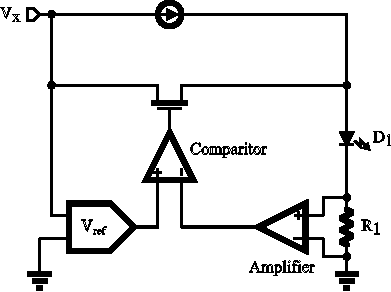
\includegraphics[width=0.6\linewidth]{3-literature/LowNoiseCurrentSourceSch.pdf}}
\caption{Low Noise Current Source Schematic}
\label{fig_LowNoiseCurrentSourceSch}
\end{figure}

A superluminescent diode is used as light source for the optrode system, which has generated most of the noise in the system.  Although there is noise generated by the superluminescent diode itself \cite{SLDNoise}, a lot of noise comes from the power source of the superluminescent diode.  An alternative way to reduce the noise from this system is to have a lower noise current source.  A low noise two-stage current source designed for laser usage \cite{LowNoiseCurrentSource} is shown in fig.~\ref{fig_LowNoiseCurrentSourceSch}, which can be similarly used on the superluminescent diode.  This design creates very low noise output current by using a normal first stage source and feedback second stage source.  The result shows that at some output levels, the noise inside the output current is low enough that it will not have a significant impact on the laser \cite{LinewidthQuantumCascadeLaser}.  Therefore, this design is suitable to power some laser diodes for high performance measurement systems.

This low noise current source design has two stages.  The first stage is a normal current source mainly made by a linear voltage regulator, and the output current can be adjusted by a trimmer.  The second stage is a negative feedback loop that provides much less amount of current than the first stage, but enough to compensate for the noise from the first stage.  The second stage consists of an amplifier, a voltage reference, and a comparator.  Both the current source outputs are connected to the anode of the laser diode, and a sense resistor is placed between the cathode of the laser diode and ground, the amplifier amplifies the voltage across the resistor, which is proportional to the laser diode current.  The amplifier output voltage is compared with a highly stable voltage reference, which is adjusted as to the desired output current.  When the amplifier output voltage is smaller than the voltage reference, that means the output current is smaller than the target current because of the noise from the first stage current source, the comparator output will turn on a MOSFET to increase the second stage current, which will compensate for the noise.  Therefore, a stable low noise current is created.

Comparing the current noise for the first stage source only and the two-stage source, at lower output of $I = \qty{200}{mA}$, the two-stage source has a noise level improvement by a factor of 10 across the frequency range from \qty{0.1}{Hz} to \qty{100}{kHz}.  However, at maximum output $I = \qty{1}{A}$, the two-stage source only improves in the frequency range from \qty{0.1}{Hz} to \qty{100}{Hz}, and it has more noise than the first stage in the frequency range from \qty{100}{Hz} to \qty{100}{kHz}.
For the current noise measurement result, the two-stage source has equivalent current noise of \qty{1.2}{nA/\sqrthz} at $I = \qty{0.2}{A}$, \qty{7.3}{nA/\sqrthz} at $I = \qty{0.5}{A}$, \qty{60}{nA/\sqrthz} at $I = \qty{1}{A}$.

At a lower output current of $I = \qty{0.2}{A}$, the \qty{1.2}{nA/\sqrthz} noise from the current source causes lower noise in the laser diode than the temperature caused noise \cite{LinewidthQuantumCascadeLaser}.  Therefore, there is no need to improve the performance at this output noise level.  However, at higher current output current levels, the noise level increases significantly.  From the spectral density result, higher current output increases the noise in the high frequency range, this might be caused by the feedback loop gain control and reaction speed, which cause the two-stage source to be less stable at higher frequencies.  One solution to this problem is to use a feedforward loop instead of a feedback loop.  By accurately sensing and calculating the noise from the first stage source, outputting this amount of current noise from the second stage source, adding both stage current and then outputting to the laser diode.  The difference between feedback and feedforward loop is that in feedforward loop, the current noise is compensated before the laser diode, and it is accurate feed, which is more stable at high frequency than the negative feedback.

This current source is designed to have an adjustable output current.  However, the adjustment is made by tuning two trimmers from the first and second stage sources.  As trimmers have no resistance mark, it is very hard to adjust them accurately.  Therefore, a microcontroller could be introduced to control the variable output current \cite{Du_2018}.  By using a microcontroller, both the speed and accuracy of setting the current output can be improved.  In the case of the feedforward loop, a microcontroller will be needed to calibrate the feedforward circuit gain to achieve better noise performance.

The sense resistor in this design is placed between the cathode of the laser diode and the ground.  This may cause the voltage across the laser diode to change along with the noisy current, which causes noise and drift for the laser diode.  This problem happens because of the feedback loop.  By changing from a feedback loop to feedforward, the current is sensed before the laser diode, which means the sense resistor will be placed between the first stage source and the anode of the laser diode, and the cathode of the laser diode will be grounded.  The ground connection issue for the amplifier can be solved by a high side sensing circuit \cite{TI_2019}.
 
In conclusion, Grzegorz presents a low noise current source design that achieves decent results of \qty{1.2}{nA/\sqrthz} noise at $I = \qty{0.2}{A}$ output, which is approaching the limit of the noise performance improvement ability of the laser diode from the current source.  However, the current source noise performance at higher output currents is less satisfying.  The feedback loop has a performance impact on higher frequency noise.  Also, the output current value takes a long time to change.  Therefore, a feed-forward current source could perform better in some aspects.



